\chapter{Complejidad temporal}

\index{complejidad temporal}

La eficiencia de los algoritmos es importante en la programación competitiva.
Por lo general, es fácil diseñar un algoritmo
que resuelve el problema lentamente,
pero el verdadero desafío es inventar un
algoritmo rápido.
Si el algoritmo es demasiado lento, obtendrá solo
puntos parciales o ningún punto en absoluto.

La \key{complejidad temporal} de un algoritmo
estima cuánto tiempo utilizará el algoritmo
para alguna entrada.
La idea es representar la eficiencia
como una función cuyo parámetro es el tamaño de la entrada.
Al calcular la complejidad temporal,
podemos averiguar si el algoritmo es lo suficientemente rápido
sin implementarlo.

\section{Reglas de cálculo}

La complejidad temporal de un algoritmo
se denota $O(\cdots)$
donde los tres puntos representan alguna
función.
Por lo general, la variable $n$ denota
el tamaño de la entrada.
Por ejemplo, si la entrada es un conjunto de números,
$n$ será el tamaño del conjunto,
y si la entrada es una cadena,
$n$ será la longitud de la cadena.

\subsubsection*{Bucles}

Una razón común por la que un algoritmo es lento es
que contiene muchos bucles que recorren la entrada.
Cuanto más bucles anidados contenga el algoritmo,
más lento será.
Si hay $k$ bucles anidados,
la complejidad temporal es $O(n^k)$.

Por ejemplo, la complejidad temporal del siguiente código es $O(n)$:
\begin{lstlisting}
for (int i = 1; i <= n; i++)
    // código
\end{lstlisting}

Y la complejidad temporal del siguiente código es $O(n^2)$:
\begin{lstlisting}
for (int i = 1; i <= n; i++)
    for (int j = 1; j <= n; j++)
        // código
\end{lstlisting}

\subsubsection*{Orden de magnitud}

Una complejidad temporal no nos dice el número exacto
de veces que se ejecuta el código dentro de un bucle,
sino que solo muestra el orden de magnitud.
En los siguientes ejemplos, el código dentro del bucle
se ejecuta $3n$, $n+5$ y $\lceil n/2 \rceil$ veces,
pero la complejidad temporal de cada código es $O(n)$.

\begin{lstlisting}
for (int i = 1; i <= 3 * n; i++) {
    // código
}
\end{lstlisting}

\begin{lstlisting}
for (int i = 1; i <= n + 5; i++) {
    // código
}
\end{lstlisting}

\begin{lstlisting}
for (int i = 1; i <= n; i += 2) {
    // código
}
\end{lstlisting}

Como otro ejemplo,
la complejidad temporal del siguiente código es $O(n^2)$:

\begin{lstlisting}
for (int i = 1; i <= n; i++) {
    for (int j = i + 1; j <= n; j++) {
        // código
    }
}
\end{lstlisting}

\subsubsection*{Fases}

Si el algoritmo consta de fases consecutivas,
la complejidad temporal total es la mayor
complejidad de todas, ya que esta
es el cuello de botella del código.

Por ejemplo, el siguiente código consta
de tres fases con complejidades temporales
$O(n)$, $O(n^2)$ y $O(n)$.
Por lo tanto, la complejidad temporal total es $O(n^2)$.

\begin{lstlisting}
for (int i = 1; i <= n; i++) {
    // código
}

for (int i = 1; i <= n; i++) {
    for (int j = 1; j <= n; j++) {
        // código
    }
}

for (int i = 1; i <= n; i++) {
    // código
}
\end{lstlisting}

\subsubsection*{Varias variables}

A veces la complejidad temporal depende de
varios factores.
En este caso, la fórmula de complejidad temporal
contiene varias variables.

Por ejemplo, la complejidad temporal del
siguiente código es $O(nm)$:

\begin{lstlisting}
for (int i = 1; i <= n; i++) {
    for (int j = 1; j <= m; j++) {
        // código
    }
}
\end{lstlisting}

\subsubsection*{Recursión}

La complejidad temporal de una función recursiva
depende del número de veces que se llama a la función
y la complejidad temporal de una sola llamada.
La complejidad temporal total es el producto de
estos valores.

Por ejemplo, considera la siguiente función:
\begin{lstlisting}
void f(int n) {
    if (n == 1) return;
    f(n - 1);
}
\end{lstlisting}
La llamada $\texttt{f}(n)$ provoca $n$ llamadas a la función,
y la complejidad temporal de cada llamada es $O(1)$.
Por lo tanto, la complejidad temporal total es $O(n)$.

Como otro ejemplo, considera la siguiente función:
\begin{lstlisting}
void g(int n) {
    if (n == 1) return;
    g(n - 1);
    g(n - 1);
}
\end{lstlisting}
En este caso, cada llamada a la función genera dos otras
llamadas, excepto para $n=1$.
Veamos qué sucede cuando se llama a $g$
con el parámetro $n$.
La siguiente tabla muestra las llamadas a la función
producidas por esta única llamada:
\begin{center}
    \begin{tabular}{rr}
        llamada a la función & número de llamadas \\
        \hline
        $g(n)$               & 1                  \\
        $g(n-1)$             & 2                  \\
        $g(n-2)$             & 4                  \\
        $\cdots$             & $\cdots$           \\
        $g(1)$               & $2^{n-1}$          \\
    \end{tabular}
\end{center}
Basándonos en esto, la complejidad temporal es
\[1+2+4+\cdots+2^{n-1} = 2^n-1 = O(2^n).\]

\section{Clases de complejidad}

\index{clases de complejidad}

La siguiente lista contiene complejidades temporales comunes
de los algoritmos:

\begin{description}
    \item[$O(1)$]
          \index{O(1)@$O(1)$}
          \index{constante (complejidad)}
          El tiempo de ejecución de un algoritmo \key{de tiempo constante}
          no depende del tamaño de la entrada.
          Un algoritmo típico de tiempo constante es una fórmula directa
          que calcula la respuesta.

    \item[$O(\log n)$]
          \index{O(log n)@$O(\log n)$}
          \index{logarítmica (complejidad)}
          Un algoritmo \key{logarítmico} a menudo reduce a la mitad
          el tamaño de la entrada en cada paso.
          Su complejidad es logarítmica porque
          $\log_2 n$ es igual al número de veces
          que $n$ debe dividirse por 2 para obtener 1.

    \item[$O(\sqrt n)$]
          \index{O(sqrt n)@$O(\sqrt n)$}
          \index{raíz cuadrada (complejidad)}
          Un \key{algoritmo de raíz cuadrada} es más lento que
          $O(\log n)$ pero más rápido que $O(n)$.
          Una propiedad especial de las raíces cuadradas es que
          $\sqrt n = n/\sqrt n$, por lo que la raíz cuadrada $\sqrt n$ se encuentra,
          en cierto sentido, en el medio de la entrada.

    \item[$O(n)$]
          \index{O(n)@$O(n)$}
          \index{lineal (complejidad)}
          Un algoritmo \key{lineal} recorre la entrada
          un número constante de veces.
          Esta es a menudo la mejor complejidad temporal posible,
          ya que generalmente es necesario acceder a cada
          elemento de entrada al menos una vez antes de
          informar la respuesta.

    \item[$O(n \log n)$]
          \index{O(n log n)@$O(n log n)$}
          \index{linearítmica (complejidad)}
          Una complejidad \key{linearítmica} a menudo indica que el
          algoritmo ordena la entrada, al ser la complejidad de
          los algoritmos de ordenamiento
          eficientes. Otra posibilidad es que el algoritmo
          utilice una estructura de datos cuyas operaciones
          tarden $O(\log n)$.

    \item[$O(n^2)$]
          \index{O(n2)@$O(n^2)$}
          \index{cuadrática (complejidad)}
          Un algoritmo \key{cuadrático} a menudo contiene
          dos bucles anidados.
          Es posible recorrer todos los pares de
          los elementos de entrada en tiempo $O(n^2)$.

    \item[$O(n^3)$]
          \index{O(n3)@$O(n^3)$}
          \index{c\'ubica (complejidad)}
          Un algoritmo \key{cúbico} a menudo contiene
          tres bucles anidados.
          Es posible recorrer todos los tríos de
          los elementos de entrada en tiempo $O(n^3)$.

    \item[$O(2^n)$]
          \index{O(2n)@$O(2^n)$}
          \index{exponencial (complejidad)}
          La complejidad \key{exponencial} a menudo indica que
          el algoritmo itera a través de todos
          los subconjuntos de los elementos de entrada.
          Por ejemplo, los subconjuntos de $\{1,2,3\}$ son
          $\emptyset$, $\{1\}$, $\{2\}$, $\{3\}$, $\{1,2\}$,
          $\{1,3\}$, $\{2,3\}$ y $\{1,2,3\}$.

    \item[$O(n!)$]
          \index{O(n!)@$O(n!)$}
          \index{factorial (complejidad)}
          La complejidad \key{factorial} a menudo indica que
          el algoritmo itera a través de todas
          las permutaciones de los elementos de entrada.
          Por ejemplo, las permutaciones de $\{1,2,3\}$ son
          $(1,2,3)$, $(1,3,2)$, $(2,1,3)$, $(2,3,1)$,
          $(3,1,2)$ y $(3,2,1)$.

\end{description}

\index{algoritmo polinomial}
Un algoritmo es \key{polinomial}
si su complejidad temporal es como máximo $O(n^k)$
donde $k$ es una constante.
Todas las complejidades temporales anteriores excepto
$O(2^n)$ y $O(n!)$ son polinomiales.
En la práctica, la constante $k$ suele ser pequeña,
y por lo tanto, una complejidad temporal polinomial
significa aproximadamente que el algoritmo es \emph{eficiente}.

\index{NP-difícil}

La mayoría de los algoritmos en este libro son polinomiales.
Sin embargo, hay muchos problemas importantes para los cuales
no se conoce ningún algoritmo polinomial, es decir,
nadie sabe cómo resolverlos de manera eficiente.
Los problemas \key{NP-difíciles} son un conjunto importante
de problemas, para los cuales no se conoce ningún algoritmo
polinomial.\footnote{Un libro clásico sobre el tema es
    \emph{Computers and Intractability: A Guide to the Theory
        of NP-Completeness} de M. R. Garey y D. S. Johnson \cite{gar79}.}

\section{Estimación de la eficiencia}

Al calcular la complejidad temporal de un algoritmo,
es posible verificar, antes de
implementar el algoritmo, que es
suficientemente eficiente para el problema.
El punto de partida para las estimaciones es el hecho de que
una computadora moderna puede realizar varios cientos de
millones de operaciones en un segundo.

Por ejemplo, supongamos que el límite de tiempo para
un problema es de un segundo y el tamaño de entrada es $n=10^5$.
Si la complejidad temporal es $O(n^2)$,
el algoritmo realizará aproximadamente $(10^5)^2=10^{10}$ operaciones.
Esto debería tomar al menos unas decenas de segundos,
por lo que el algoritmo parece ser demasiado lento para resolver el problema.

Por otro lado, dado el tamaño de entrada,
podemos intentar \emph{adivinar}
la complejidad temporal requerida del algoritmo
que resuelve el problema.
La siguiente tabla contiene algunas estimaciones útiles
suponiendo un límite de tiempo de un segundo.

\begin{center}
    \begin{tabular}{ll}
        tamaño de entrada & complejidad temporal requerida \\
        \hline
        $n \le 10$        & $O(n!)$                        \\
        $n \le 20$        & $O(2^n)$                       \\
        $n \le 500$       & $O(n^3)$                       \\
        $n \le 5000$      & $O(n^2)$                       \\
        $n \le 10^6$      & $O(n \log n)$ o $O(n)$         \\
        $n$ es grande     & $O(1)$ o $O(\log n)$           \\
    \end{tabular}
\end{center}

Por ejemplo, si el tamaño de entrada es $n=10^5$,
probablemente se espera que la complejidad
temporal del algoritmo sea $O(n)$ o $O(n \log n)$.
Esta información facilita el diseño del algoritmo,
porque descarta enfoques que generarían
un algoritmo con una peor complejidad temporal.

\index{factor constante}

Aun así, es importante recordar que una
complejidad temporal es solo una estimación de la eficiencia,
porque oculta los \emph{factores constantes}.
Por ejemplo, un algoritmo que se ejecuta en tiempo $O(n)$
puede realizar $n/2$ o $5n$ operaciones.
Esto tiene un efecto importante en el tiempo de ejecución
real del algoritmo.

\section{Subarreglo de suma máxima}

\index{subarreglo de suma máxima}
\index{suma máxima en subarreglo}

A menudo hay varios algoritmos posibles
para resolver un problema de manera que sus
complejidades temporales sean diferentes.
Esta sección analiza un problema clásico que
tiene una solución directa de $O(n^3)$.
Sin embargo, al diseñar un algoritmo mejor, es
posible resolver el problema en tiempo $O(n^2)$
e incluso en tiempo $O(n)$.

Dado un arreglo de $n$ números,
nuestra tarea es calcular el
\key{suma máxima en subarreglo}, es decir,
la suma más grande posible de
una secuencia de valores consecutivos
en el arreglo.\footnote{El libro de J. Bentley
    \emph{Programming Pearls} \cite{ben86} hizo popular el problema.}
El problema se hace interesante cuando puede haber
valores negativos en el arreglo.
Por ejemplo, en el arreglo
\begin{center}
    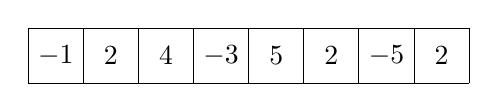
\begin{tikzpicture}[scale=0.7]
        \draw (0,0) grid (8,1);

        \node at (0.5,0.5) {$-1$};
        \node at (1.5,0.5) {$2$};
        \node at (2.5,0.5) {$4$};
        \node at (3.5,0.5) {$-3$};
        \node at (4.5,0.5) {$5$};
        \node at (5.5,0.5) {$2$};
        \node at (6.5,0.5) {$-5$};
        \node at (7.5,0.5) {$2$};
    \end{tikzpicture}
\end{center}
\begin{samepage}
    el siguiente subarreglo produce la suma máxima $10$:
    \begin{center}
        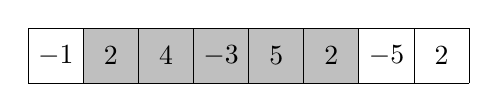
\begin{tikzpicture}[scale=0.7]
            \fill[color=lightgray] (1,0) rectangle (6,1);
            \draw (0,0) grid (8,1);

            \node at (0.5,0.5) {$-1$};
            \node at (1.5,0.5) {$2$};
            \node at (2.5,0.5) {$4$};
            \node at (3.5,0.5) {$-3$};
            \node at (4.5,0.5) {$5$};
            \node at (5.5,0.5) {$2$};
            \node at (6.5,0.5) {$-5$};
            \node at (7.5,0.5) {$2$};
        \end{tikzpicture}
    \end{center}
\end{samepage}

Asumimos que se permite un subarreglo vacío,
así que la suma máxima en subarreglo es siempre al menos $0$.

\subsubsection{Algoritmo 1}

Una forma sencilla de resolver el problema
es recorrer todos los subarreglos posibles,
calcular la suma de valores en cada subarreglo y mantener
la suma máxima.
El siguiente código implementa este algoritmo:

\begin{lstlisting}
int mejor = 0;
for (int a = 0; a < n; a++) {
    for (int b = a; b < n; b++) {
        int suma = 0;
        for (int k = a; k <= b; k++)
            suma += arreglo[k];
        mejor = max(mejor, suma);
    }
}
cout << mejor << "\n";
\end{lstlisting}

Las variables \texttt{a} y \texttt{b} fijan el primer y
último índice del subarreglo,
y la suma de valores se calcula en la variable \texttt{suma}.
La variable \texttt{mejor} contiene la suma máxima encontrada durante la búsqueda.

La complejidad temporal del algoritmo es $O(n^3)$,
porque consiste en tres bucles anidados
que recorren la entrada.

\subsubsection{Algoritmo 2}

Es fácil hacer el Algoritmo 1 más eficiente
eliminando un bucle de él.
Esto es posible calculando la suma al mismo
tiempo que se mueve el extremo derecho del subarreglo.
El resultado es el siguiente código:

\begin{lstlisting}
int mejor = 0;
for (int a = 0; a < n; a++) {
    int suma = 0;
    for (int b = a; b < n; b++) {
        suma += arreglo[b];
        mejor = max(mejor,suma);
    }
}
cout << mejor << "\n";
\end{lstlisting}
Después de este cambio, la complejidad en tiempo es $O(n^2)$.

\subsubsection{Algoritmo 3}

\index{algoritmo de Kadane}

Sorprendentemente, es posible resolver el problema
en tiempo $O(n)$,\footnote{En \cite{ben86} este algoritmo de tiempo lineal
    se atribuye a J. B. Kadane, y el algoritmo a veces se
    llama \key{algoritmo de Kadane}.}, lo que significa
que solo se necesita un bucle.
La idea es calcular, para cada posición del arreglo,
la suma máxima de un subarreglo que termina en esa posición.
Después de esto, la respuesta al problema es el
máximo de esas sumas.

Consideremos el subproblema de encontrar el subarreglo de suma máxima
que termina en la posición $k$.
Hay dos posibilidades:
\begin{enumerate}
    \item El subarreglo solo contiene el elemento en la posición $k$.
    \item El subarreglo consta de un subarreglo que termina
          en la posición $k-1$, seguido del elemento en la posición $k$.
\end{enumerate}

En el último caso, dado que queremos
encontrar un subarreglo con suma máxima,
el subarreglo que termina en la posición $k-1$
también debe tener la suma máxima.
Por lo tanto, podemos resolver el problema de manera eficiente
calculando la suma de subarreglos máxima
para cada posición final de izquierda a derecha.

El siguiente código implementa el algoritmo:
\begin{lstlisting}
int mejor = 0, suma = 0;
for (int k = 0; k < n; k++) {
    suma = max(arreglo[k], suma + arreglo[k]);
    mejor = max(mejor, suma);
}
cout << best << "\n";
\end{lstlisting}

El algoritmo solo contiene un bucle
que recorre la entrada,
por lo que su complejidad temporal es $O(n)$.
Esta también es la mejor complejidad posible,
porque cualquier algoritmo para el problema
tiene que examinar todos los elementos del arreglo al menos una vez.

\subsubsection{Comparación de eficiencia}

Es interesante estudiar qué tan eficientes
son los algoritmos en la práctica.
La siguiente tabla muestra los tiempos de ejecución
de los algoritmos anteriores para diferentes
valores de $n$ en una computadora moderna.

En cada prueba, la entrada se generó al azar.
El tiempo necesario para leer la entrada no fue
medido.

\begin{center}
    \begin{tabular}{rrrr}
        tamaño del arreglo $n$ & Algoritmo 1 & Algoritmo 2 & Algoritmo 3 \\
        \hline
        $10^2$                 & $0.0$ s     & $0.0$ s     & $0.0$ s     \\
        $10^3$                 & $0.1$ s     & $0.0$ s     & $0.0$ s     \\
        $10^4$                 & > $10.0$ s  & $0.1$ s     & $0.0$ s     \\
        $10^5$                 & > $10.0$ s  & $5.3$ s     & $0.0$ s     \\
        $10^6$                 & > $10.0$ s  & > $10.0$ s  & $0.0$ s     \\
        $10^7$                 & > $10.0$ s  & > $10.0$ s  & $0.0$ s     \\
    \end{tabular}
\end{center}

La comparación muestra que todos los algoritmos
son eficientes cuando el tamaño de la entrada es pequeño,
pero las entradas más grandes resaltan diferencias notables
en los tiempos de ejecución de los algoritmos.
El Algoritmo 1 se vuelve lento
cuando $n=10^4$, y el Algoritmo 2
se vuelve lento cuando $n=10^5$.
Solo el Algoritmo 3 es capaz de procesar
incluso las entradas más grandes al instante.
